% idea-to-paper skeleton (IEEE conference). Copy into the paper folder, then replace every <<FILL: ...>> line and every DEMO block.
% check_paper.py fails while any <<FILL or ">>> DEMO" marker remains. Keep one paragraph per line.
\documentclass[conference]{IEEEtran}
\IEEEoverridecommandlockouts
\usepackage[T1]{fontenc}
\usepackage{cite}
\usepackage{amsmath,amssymb,amsfonts}
\usepackage{algorithm}
\usepackage{algpseudocode}
\usepackage{graphicx}
\usepackage{textcomp}
\usepackage{xcolor}
\usepackage{booktabs}
\usepackage{multirow}
\usepackage{url}
\usepackage{fontawesome5}
\usepackage{tikz}
\usetikzlibrary{positioning,arrows.meta,fit,backgrounds,calc}
\usepackage{pgfplots}
\pgfplotsset{compat=1.18}

% ---------- Implementation targets (never recolor, hide, or redefine these) ----------
% IMPLEMENTATION TARGETS: blue values are planned outcomes of the experimental protocol, not measurements.
\definecolor{tgtblue}{RGB}{0,82,204}
\newcommand{\tgt}[1]{\textcolor{tgtblue}{#1}}
\newcommand{\tgtcap}{\textcolor{tgtblue}{[Implementation target]}~}
\newcommand{\tgtnotice}{Values in blue are implementation targets. They state the outcomes the experimental protocol is designed to reach and are not measured results. Each must be replaced with its measured value before submission.}

% ---------- Figure palette: pastel fills, Okabe-Ito plot colors ----------
\definecolor{boxA}{RGB}{220,234,247}
\definecolor{boxB}{RGB}{226,240,217}
\definecolor{boxC}{RGB}{252,228,214}
\definecolor{boxD}{RGB}{234,224,244}
\definecolor{boxE}{RGB}{255,242,204}
\definecolor{lineC}{RGB}{70,80,95}
\definecolor{plotA}{RGB}{0,114,178}
\definecolor{plotB}{RGB}{230,159,0}
\definecolor{plotC}{RGB}{0,158,115}
\definecolor{plotD}{RGB}{213,94,0}
\definecolor{plotE}{RGB}{204,121,167}
\tikzset{
  blk/.style={draw=lineC, rounded corners=3pt, align=center, font=\footnotesize, minimum height=7mm, inner sep=3pt, line width=0.5pt},
  flow/.style={-{Stealth[length=2mm]}, draw=lineC, line width=0.6pt},
  dflow/.style={flow, dashed},
  grp/.style={draw=lineC!60, rounded corners=5pt, dashed, inner sep=5pt},
  lbl/.style={font=\scriptsize, text=lineC},
}
\pgfplotsset{
  ieee/.style={width=\columnwidth, height=4.4cm, font=\footnotesize, tick label style={font=\scriptsize}, label style={font=\footnotesize}, legend style={font=\scriptsize, draw=none, fill=none}, grid=major, grid style={gray!25}, axis line style={lineC}},
}

\title{<<FILL: paper title>>\thanks{\textcolor{tgtblue}{\tgtnotice}}}
\author{\IEEEauthorblockN{Anonymous Author(s)}
\IEEEauthorblockA{Affiliation withheld for double-anonymous review}}

\begin{document}
\maketitle

\begin{abstract}
<<FILL: abstract, 150 to 250 words, one paragraph on one line, every unmeasured number wrapped in the tgt macro>>
\end{abstract}

\begin{IEEEkeywords}
<<FILL: four to six keywords, comma separated>>
\end{IEEEkeywords}

\section{Introduction}\label{sec:intro}
<<FILL: motivation paragraph with a concrete problem, scale, and cost, supported by citations such as \cite{he2016deep}>>

<<FILL: research gap paragraph that names what prior work leaves open and why it matters>>

<<FILL: one sentence that introduces the contribution list>>
\begin{itemize}
\item <<FILL: contribution 1, one line, names the artifact and where it appears (Section~\ref{sec:method})>>
\item <<FILL: contribution 2>>
\item <<FILL: contribution 3, evaluation contribution that points to Section~\ref{sec:results}>>
\end{itemize}

\section{Related Work}\label{sec:related}
\subsection{<<FILL: theme 1>>}
<<FILL: synthesis paragraph comparing approaches, not a list of summaries>>

\subsection{<<FILL: theme 2>>}
<<FILL: synthesis paragraph that ends with the gap this paper fills, summarized in Table~\ref{tab:related}>>

% >>> DEMO related-work comparison table: one row per verified prior work, columns are the paper's design dimensions
\begin{table}[t]
\centering
\caption{Comparison of representative prior work with the proposed framework.}
\label{tab:related}
% CONFIG: qualitative comparison derived from the cited papers
\setlength{\tabcolsep}{3.5pt}
\begin{tabular}{@{}lcccc@{}}
\toprule
Work & Privacy & Trust & Real-time & Explainable \\
\midrule
He et al.~\cite{he2016deep} & $\times$ & $\times$ & \checkmark & $\times$ \\
Kingma and Ba~\cite{kingma2014adam} & $\times$ & $\times$ & $\times$ & $\times$ \\
Proposed & \checkmark & \checkmark & \checkmark & \checkmark \\
\bottomrule
\end{tabular}
\end{table}
% <<< DEMO

\section{Proposed Framework}\label{sec:method}
<<FILL: design goals and assumptions, threat model when security is in scope>>

<<FILL: overview of the method in prose, pointing to the workflow in Fig.~\ref{fig:workflow}>>

% >>> DEMO workflow loop figure (column width)
\begin{figure}[t]
\centering
\begin{tikzpicture}[node distance=5mm]
\node[blk, fill=boxA, text width=13mm] (obs) {\faEye\\[1pt] Observe};
\node[blk, fill=boxB, text width=13mm, right=of obs] (plan) {\faBrain\\[1pt] Plan};
\node[blk, fill=boxC, text width=13mm, right=of plan] (act) {\faCogs\\[1pt] Act};
\node[blk, fill=boxD, text width=13mm, right=of act] (ver) {\faCheckCircle\\[1pt] Verify};
\draw[flow] (obs) -- (plan);
\draw[flow] (plan) -- (act);
\draw[flow] (act) -- (ver);
\draw[dflow] (ver.south) -- ++(0,-5mm) -| node[lbl, pos=0.25, below]{feedback updates the policy} (obs.south);
\end{tikzpicture}
\caption{Closed-loop workflow. Each cycle observes the environment, plans an action, executes it, and verifies the outcome before the next cycle.}
\label{fig:workflow}
\end{figure}
% <<< DEMO

\section{System Architecture}\label{sec:arch}
<<FILL: walk through each component of Fig.~\ref{fig:architecture} in the order data flows through it>>

% >>> DEMO architecture figure (full width): replace every node with the paper's own components
\begin{figure*}[t]
\centering
\begin{tikzpicture}[node distance=6mm and 13mm]
\node[blk, fill=boxA, text width=21mm] (src) {\faDatabase\\[2pt] \textbf{Data Sources}\\ sensors and logs};
\node[blk, fill=boxB, text width=21mm, right=of src] (edge) {\faMicrochip\\[2pt] \textbf{Edge Agents}\\ local training};
\node[blk, fill=boxC, text width=21mm, right=of edge] (coord) {\faProjectDiagram\\[2pt] \textbf{Coordinator}\\ aggregation};
\node[blk, fill=boxD, text width=21mm, right=of coord] (gov) {\faUserShield\\[2pt] \textbf{Governance}\\ trust scoring};
\node[blk, fill=boxE, text width=21mm, right=of gov] (app) {\faChartLine\\[2pt] \textbf{Applications}\\ decisions};
\draw[flow] (src) -- node[lbl, above]{raw data} (edge);
\draw[flow] (edge) -- node[lbl, above]{updates} (coord);
\draw[flow] (coord) -- node[lbl, above]{model} (gov);
\draw[flow] (gov) -- node[lbl, above]{verified} (app);
\draw[dflow] (gov.south) -- ++(0,-7mm) -| node[lbl, pos=0.25, below]{policy feedback to agents} (edge.south);
\begin{scope}[on background layer]
\node[grp, fit=(edge)(coord)(gov), label={[lbl]above:trusted execution zone}] {};
\end{scope}
\end{tikzpicture}
\caption{Architecture of the proposed framework. Solid arrows carry data and model updates, and the dashed arrow carries governance feedback to the edge agents.}
\label{fig:architecture}
\end{figure*}
% <<< DEMO

\section{Mathematical Model and Algorithms}\label{sec:model}
\subsection{Problem Formulation}
<<FILL: define the system, sets, and variables before any equation uses them>>

% >>> DEMO equation: every numbered equation gets a label and an in-text reference
\begin{equation}
\mathcal{L}(\theta) = \frac{1}{|\mathcal{D}|}\sum_{(x,y)\in\mathcal{D}} \ell\big(f_\theta(x), y\big) + \lambda \lVert \theta \rVert_2^2
\label{eq:loss}
\end{equation}
% <<< DEMO
<<FILL: sentence that explains each symbol in Equation~\eqref{eq:loss}>>

\subsection{Algorithm}
<<FILL: describe Algorithm~\ref{alg:main} and state its time and communication complexity>>

% >>> DEMO algorithm
\begin{algorithm}[t]
\caption{Training procedure}
\label{alg:main}
\begin{algorithmic}[1]
\Require Dataset $\mathcal{D}$, rounds $T$, learning rate $\eta$
\Ensure Model parameters $\theta_T$
\State Initialize $\theta_0$
\For{$t = 0$ to $T-1$}
\State Sample a mini-batch $\mathcal{B}_t \subset \mathcal{D}$
\State $\theta_{t+1} \gets \theta_t - \eta \nabla_\theta \mathcal{L}(\theta_t; \mathcal{B}_t)$
\EndFor
\State \Return $\theta_T$
\end{algorithmic}
\end{algorithm}
% <<< DEMO

\section{Experimental Setup}\label{sec:setup}
<<FILL: datasets with verified statistics and citations, splits, baselines, metrics, hardware wrapped in the tgt macro, and seeds, with hyperparameters in Table~\ref{tab:hyper}>>

% >>> DEMO hyperparameter table (a configuration, not a result)
\begin{table}[t]
\centering
\caption{Training configuration.}
\label{tab:hyper}
% CONFIG: design choices of the experimental protocol
\begin{tabular}{@{}ll@{}}
\toprule
Parameter & Value \\
\midrule
Optimizer & Adam~\cite{kingma2014adam} \\
Learning rate & $1\times10^{-3}$ \\
Batch size & 64 \\
Epochs & 100 \\
\bottomrule
\end{tabular}
\end{table}
% <<< DEMO

\section{Results and Discussion}\label{sec:results}
<<FILL: main result with the number and its comparison point, for example an F1-score of \tgt{92.2}\% against \tgt{90.0}\% for the strongest baseline in Table~\ref{tab:main} and Fig.~\ref{fig:bars}>>

% >>> DEMO main comparison table: F1 must equal 2PR/(P+R) for every row unless the caption says macro-averaged
\begin{table}[t]
\centering
\caption{\tgtcap Detection performance on the test split (mean over five seeds).}
\label{tab:main}
\setlength{\tabcolsep}{4pt}
\begin{tabular}{@{}lcccc@{}}
\toprule
Method & Precision (\%) & Recall (\%) & F1 (\%) & Latency (ms) \\
\midrule
Baseline A & \tgt{88.1} & \tgt{85.4} & \tgt{86.7} & \tgt{41.2} \\
Baseline B & \tgt{89.6} & \tgt{87.9} & \tgt{88.7} & \tgt{38.5} \\
Baseline C & \tgt{90.8} & \tgt{89.2} & \tgt{90.0} & \tgt{52.9} \\
Proposed & \textbf{\tgt{92.7}} & \textbf{\tgt{91.7}} & \textbf{\tgt{92.2}} & \tgt{44.6} \\
\bottomrule
\end{tabular}
\end{table}
% <<< DEMO

% >>> DEMO grouped comparison bar chart (values match Table tab:main)
\begin{figure}[t]
\centering
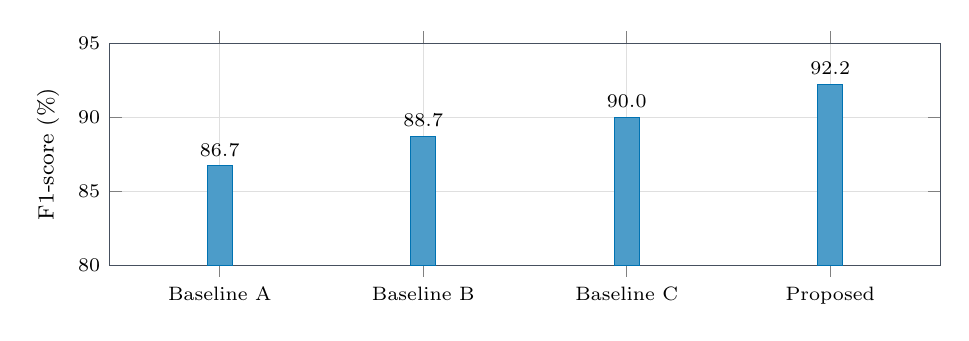
\begin{tikzpicture}
\begin{axis}[ieee, ybar, bar width=9pt, ymin=80, ymax=95, ylabel={F1-score (\%)}, symbolic x coords={Baseline A,Baseline B,Baseline C,Proposed}, xtick=data, nodes near coords={\pgfmathprintnumber[fixed,fixed zerofill,precision=1]{\pgfplotspointmeta}}, nodes near coords style={font=\scriptsize}, enlarge x limits=0.18]
\addplot[fill=plotA!70, draw=plotA] coordinates {(Baseline A,86.7) (Baseline B,88.7) (Baseline C,90.0) (Proposed,92.2)};
\end{axis}
\end{tikzpicture}
\caption{\tgtcap F1-score of each method on the test split.}
\label{fig:bars}
\end{figure}
% <<< DEMO

<<FILL: convergence or learning-curve paragraph that reads Fig.~\ref{fig:curve}>>

% >>> DEMO line plot (final points match Table tab:main)
\begin{figure}[t]
\centering
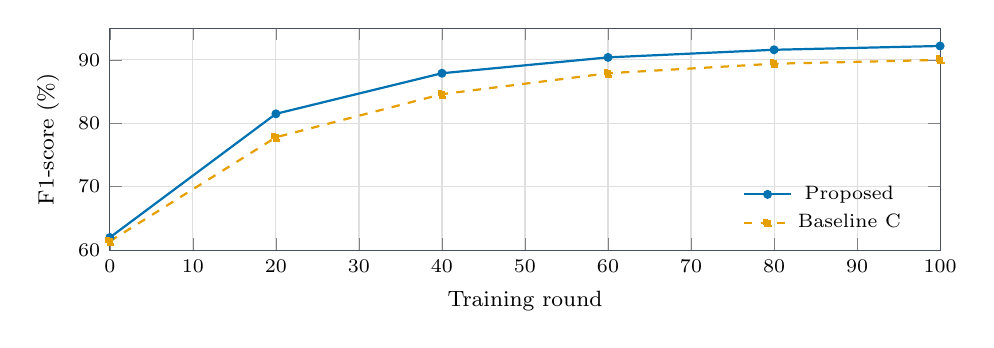
\begin{tikzpicture}
\begin{axis}[ieee, xlabel={Training round}, ylabel={F1-score (\%)}, xmin=0, xmax=100, ymin=60, ymax=95, legend pos=south east]
\addplot[plotA, thick, mark=*, mark size=1.2pt] coordinates {(0,62.0) (20,81.5) (40,87.9) (60,90.4) (80,91.6) (100,92.2)};
\addplot[plotB, thick, dashed, mark=square*, mark size=1.2pt] coordinates {(0,61.4) (20,77.8) (40,84.6) (60,87.9) (80,89.4) (100,90.0)};
\legend{Proposed, Baseline C}
\end{axis}
\end{tikzpicture}
\caption{\tgtcap F1-score per training round for the proposed method and the strongest baseline.}
\label{fig:curve}
\end{figure}
% <<< DEMO

\subsection{Ablation Study}
<<FILL: ablation paragraph that names the component whose removal costs the most, reading Table~\ref{tab:ablation} and Fig.~\ref{fig:confusion}>>

% >>> DEMO ablation table (the full model row matches Table tab:main)
\begin{table}[t]
\centering
\caption{\tgtcap Ablation of the framework components (F1, \%).}
\label{tab:ablation}
\begin{tabular}{@{}lc@{}}
\toprule
Variant & F1 (\%) \\
\midrule
Full model & \textbf{\tgt{92.2}} \\
Without component A & \tgt{90.4} \\
Without component B & \tgt{89.8} \\
Without component C & \tgt{91.0} \\
\bottomrule
\end{tabular}
\end{table}
% <<< DEMO

% >>> DEMO confusion matrix (row-normalized: rows sum to 1, mean diagonal 0.917 matches the 91.7 recall in Table tab:main)
\begin{figure}[t]
\centering
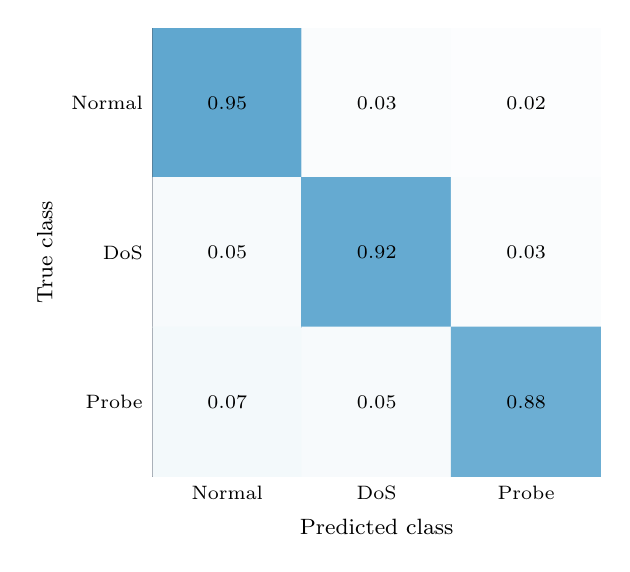
\begin{tikzpicture}
\begin{axis}[ieee, width=0.6\columnwidth, height=0.6\columnwidth, grid=none, enlargelimits=false, colormap={soft}{color=(white) color=(plotA!65)}, point meta min=0, point meta max=1, xtick={0,1,2}, ytick={0,1,2}, xticklabels={Normal,DoS,Probe}, yticklabels={Normal,DoS,Probe}, xlabel={Predicted class}, ylabel={True class}, y dir=reverse, nodes near coords={\pgfmathprintnumber[fixed,fixed zerofill,precision=2]{\pgfplotspointmeta}}, nodes near coords style={font=\scriptsize, anchor=center}]
\addplot[matrix plot*, mesh/cols=3, point meta=explicit] table[meta=v] {
x y v
0 0 0.95
1 0 0.03
2 0 0.02
0 1 0.05
1 1 0.92
2 1 0.03
0 2 0.07
1 2 0.05
2 2 0.88
};
\end{axis}
\end{tikzpicture}
\caption{\tgtcap Row-normalized confusion matrix of the proposed method on the test split.}
\label{fig:confusion}
\end{figure}
% <<< DEMO

\section{Comparative Analysis}\label{sec:compare}
<<FILL: compare against the strongest prior systems on accuracy, cost, and assumptions, including where the proposed method is worse>>

\section{Limitations}\label{sec:limits}
<<FILL: concrete limitations tied to the design and evaluation, not generic caveats>>

\section{Conclusion and Future Work}\label{sec:conclusion}
<<FILL: what the paper showed, with the headline number, and two or three specific next steps>>

\bibliographystyle{IEEEtran}
\bibliography{references}

\end{document}
